\documentclass[german,11pt]{beamer}
% ------------------------------------------------------------------------------
% Packages
\usepackage[german,english,french]{babel}
\usepackage[T1]{fontenc}
\usepackage[utf8]{inputenc}
\usepackage{ragged2e}
\usepackage[normalem]{ulem}


\usepackage{listings}
\usepackage{color}
\usepackage{xcolor} 
\usepackage{plantuml}
% \usepackage{enumitem} \setitemize{leftmargin=*}   // Keine Aufzählung
\usepackage{pgfplots}

\usepackage{csquotes}

\pgfplotsset{compat=1.18}

\definecolor{dkgreen} {rgb}{0,0.6,0}
\definecolor{gray}{rgb}{0.5,0.5,0.5}
\definecolor{mauve}{rgb}{0.58,0,0.82}

\lstset{frame=tb,
  language=Java,
  aboveskip=3mm,
  belowskip=3mm,
  showstringspaces=false,
  columns=flexible,
  basicstyle={\small\ttfamily},
  numbers=none,
  numberstyle=\tiny\color{gray},
  keywordstyle=\color{blue},
  commentstyle=\color{dkgreen},
  stringstyle=\color{mauve},
  breaklines=true,
  breakatwhitespace=true,
  tabsize=3
}
% ------------------------------------------------------------------------------
% Parameters
\mode<presentation>{\usetheme{Luebeck}}
\setbeamertemplate{itemize items}[triangle]
\setbeamercovered{transparent}
\usecolortheme{dove}
\usefonttheme{serif}
\addtobeamertemplate{block begin}{}{\justifying}
% ToC
\AtBeginSection[] {
  \begin{frame}{Inhalt}
    \tableofcontents[currentsection]
  \end{frame}
}
% Headline
\makeatletter
\setbeamertemplate{headline}{%
  \leavevmode%
  \@tempdimb=2.4375ex%
  \ifnum\beamer@subsectionmax<\beamer@sectionmax%
    \multiply\@tempdimb by\beamer@sectionmax%
  \else%
    \multiply\@tempdimb by\beamer@subsectionmax%
  \fi%
  \ifdim\@tempdimb>0pt%
    \advance\@tempdimb by 1.825ex%
    \begin{beamercolorbox}[wd=.5\paperwidth,ht=\@tempdimb]{section in head/foot}%
      \vbox to\@tempdimb{\hfill\insertsectionnavigation{.3\paperwidth}\vfil}%
    \end{beamercolorbox}%
    \begin{beamercolorbox}[wd=.3\paperwidth,ht=\@tempdimb]{subsection in head/foot}%
      \vbox to\@tempdimb{\vfil\insertsubsectionnavigation{.5\paperwidth}\vfil}%
    \end{beamercolorbox}%
    \begin{beamercolorbox}[wd=.2\paperwidth,ht=\@tempdimb]{subsection in head/foot}%
      \vbox to\@tempdimb{\vfil\hfill
\includegraphics[height=1cm]{fig/graphics/logo.jpg}\vfil}
    \end{beamercolorbox}%    
  \fi%
}
\makeatother
% Footline
\makeatletter
\setbeamertemplate{footline}{%
  \leavevmode%
  \hbox{\begin{beamercolorbox}[wd=.5\paperwidth,ht=2.5ex,dp=1.125ex,leftskip=.3cm,rightskip=.3cm]{author in head/foot}%
    \usebeamerfont{author in head/foot}\insertshortdate \hfill \insertshortauthor
  \end{beamercolorbox}%
  \begin{beamercolorbox}[wd=.5\paperwidth,ht=2.5ex,dp=1.125ex,leftskip=.3cm,rightskip=.3cm plus1fil]{title in head/foot}%
    \usebeamerfont{title in head/foot}\insertshorttitle \hfill \insertframenumber\,/\,\inserttotalframenumber
  \end{beamercolorbox}}%
  \vskip0pt%
}
\makeatother

\addto\captionsenglish{% Replace "english" with the language you use
  \renewcommand{\contentsname}%
    {Whatever}%
}

% ------------------------------------------------------------------------------
% Infos
\title[VS]{Verteilte Systeme}
%\subtitle[Short subtitle]{Subtitle}
\author[BCK]{Prof. Dr. Martin Becke}
\date[0.9]{Version 0.9}
\institute[CaDS]{CaDS - HAW Hamburg}
%\logo{
\includegraphics[height=1cm]{fig/graphics/logo.jpg}}
% ------------------------------------------------------------------------------

% Document
\begin{document}

% ------------------------------------------------------------------------------
% Titlepage
\begin{frame}
  \titlepage{}
\end{frame}
% ------------------------------------------------------------------------------
% ToC
%\begin{frame}{Contents}
%  \tableofcontents
%\end{frame}
% ------------------------------------------------------------------------------

\section{Architektur}
%\subsection{Einleitung}
\begin{frame}
  \frametitle{Architektur in Verteilten Systemen}
  \framesubtitle{Allgemein}
  \begin{itemize}
    \item Freiheitsgrade der Realisierung
    \item Am Ende Aufruf ISA der Architekturen
    \item Notwendigkeit der Kommunikation
    \item Zerlegung beherrschbar durch Zerlegungsmethoden
  \end{itemize}
\end{frame}

%\subsection{Einleitung}
\begin{frame}
  \frametitle{Zerlegungsmethoden}
  \framesubtitle{Teile-und-Herrsche-Strategie}
  \begin{itemize}
    \item Funktional
    \item Ressourcenorientiert
  \end{itemize}
\end{frame}

\begin{frame}
  \frametitle{Zerlegungsmethoden}
  \framesubtitle{Funktional}
  \begin{itemize}
    \item Kleinere, im besten Fall atomare, Funktionen/Prozeduren
    \item Funktionen sind von einander unabhängig
    \item Sprachen theoretisch austauschbar (Sprachen Turing-vollständig)
    \item Kosten: Zeit und Speicher
  \end{itemize} 
\end{frame}

\begin{frame}
  %\frametitle{Zerlegungsmethoden}
  \framesubtitle{Funktional}
  \begin{itemize}
    \item Funktionssignatur
    \begin{itemize}
      \item Name
      \item Parameter
      \item Rückgabetyp
      \item Bedingungen/Einschränkungen
     \end{itemize} 
    \item Funktionssemantik/-Definition
    \begin{itemize}
      \item Ausführungslogik
      \item Fehlerbehandlung
      \item Beschreibung durch Kommentare, Dokumentation oder Code
    \end{itemize} 
  \end{itemize} 
\end{frame}

\begin{frame}[fragile]
  %\frametitle{Zerlegungsmethoden}
  %\noindent\begin{minipage}{\textwidth}
  \framesubtitle{Funktional - Beispiel}
  \begin{lstlisting}[caption={Funktionssignatur},captionpos=b,label={lst:signatur}]
    function sum(a: int, b: int) -> int;
  \end{lstlisting}

  \begin{lstlisting}[caption={Funktionssemantik},captionpos=b,label={lst:semantik}]
    function sum(a: int, b: int) -> int {
        return a + b;
    }
  \end{lstlisting}
  %\end{minipage}
\end{frame}

\begin{frame}
  %\frametitle{Zerlegungsmethoden}
  \framesubtitle{Ressourcenorientiert}
  \begin{itemize}
    \item Kleinere, auf Ressourcen orientierte Sicht 
    \item Einheit auf eine bestimmte Ressource spezialisiert
    \item Nur Set von Funktionen: Basis CRUD
    \item Häufig intuitiver als Funktionen
  \end{itemize} 
\end{frame}


\begin{frame}
  %\frametitle{Zerlegungsmethoden}
  \framesubtitle{Beispiel Stuhl}
  \begin{figure}[ht]
  \centering
  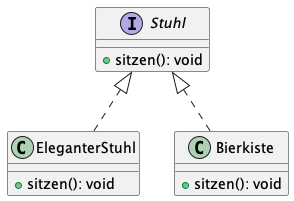
\includegraphics[width=0.3\textwidth]{fig/uml/stuhl-function.png}
  \caption{Funktionale Zerlegung mit Interface}
  \label{fig:stuhl-f}
  \end{figure}
  \begin{figure}[ht]
  \centering
  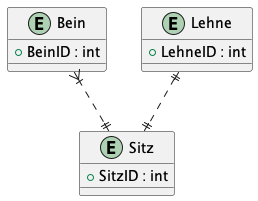
\includegraphics[width=0.3\textwidth]{fig/uml/stuhl-resourcen.png}
  \caption{Ressourcen-orientierte Zerlegung mit Relation}
  \label{fig:stuhl-r}
  \end{figure}
\end{frame}

\begin{frame}[fragile]
  %\frametitle{Zerlegungsmethoden}
  \noindent\begin{minipage}{\textwidth}
  \framesubtitle{Beispiel Schach in Code}
    \begin{lstlisting}[caption={Schachbrett - Objektorientiert},captionpos=b,label={lst:schachbrett-oo}]
    public class ChessBoard {
        private Piece[][] board;

        public ChessBoard() {
            this.board = new Piece[8][8];
            // Initialize the board with the starting positions of pieces
            // e.g. add new Piece(PieceType.ROOK, Color.WHITE) to board[0][0] for the white rook in the top-left corner.
        }

        public void setPiece(int row, int col, Piece piece) {
            board[row][col] = piece;
        }
    }
  \end{lstlisting}
  \end{minipage}
\end{frame}

\begin{frame}[fragile]
  \begin{lstlisting}[caption={Schachbrett - Datenbank},captionpos=b,label={lst:schachbrett-datenbank}]

  CREATE TABLE ChessBoard (
      id INT PRIMARY KEY,
      row INT,
      col INT,
      pieceType VARCHAR(10),
      pieceColor VARCHAR(5)
  );
\end{lstlisting}
\end{frame}

\subsection{Datenseparation}
\begin{frame}
  \frametitle{Datenseperation}
  \framesubtitle{Einführung}
  \begin{itemize}
    \item Daten auf mehreren Knoten in einem Netzwerk
    \item Aufteilung von Daten in kleine Teile
    \item Verschiedene Methoden
  \end{itemize}
\end{frame}

\begin{frame}
  \frametitle{Datenseperation}
  \framesubtitle{Methoden}
  \begin{itemize}
    \item Horizontale Partitionierung
    \item Vertikale Partitionierung
    \item Sharding
    \item Replikation
  \end{itemize}
\end{frame}
\section{Kommunikation}
%\subsection{Einleitung}
\begin{frame}
  \frametitle{Kommunikation}
  \framesubtitle{Schnittstellen}
  \begin{itemize}
    \item Datenaustausch
    \item Ressourcenmanagement
    \item Koordination
    \item Fehlererkennung und -behebung
    \item Skalierung
  \end{itemize}
\end{frame}

\begin{frame}
  \frametitle{Kommunikation}
  \framesubtitle{Art}
  \begin{itemize}
    \item Synchrone Kommunikation
    \item Asynchrone Kommunikation
  \end{itemize}
\end{frame}

\begin{frame}
  \frametitle{Kommunikation}
  \framesubtitle{Art}
  \begin{itemize}
    \item Persistente Kommunikation
    \item Transiente Kommunikation
  \end{itemize}
\end{frame}

\begin{frame}
  \frametitle{Kommunikation}
  \framesubtitle{Art}
  \begin{itemize}
    \item Signal
    \item Event
    \item Nachricht
  \end{itemize}
\end{frame}
%\section{Einleitung}
\subsection{Kopplung}
\begin{frame}
  \frametitle{Kopplung}
  \framesubtitle{Idee}
  \begin{itemize}
    \item Art und Weise wie interagiert und kommuniziert wird
    \item Wahl der Kopplungsart wesentlich für Aufbau und Leistung
    \item Starker Einfluss auf Interoperabilität und Integration
  \end{itemize}
\end{frame}

\begin{frame}
  \frametitle{Kopplung}
  \framesubtitle{Arten}
  \begin{itemize}
    \item Direkte Kopplung
    \begin{itemize}
      \item Mediator-System
      \item Middleware
    \end{itemize}
    \item Indirekte Kopplung
    \item Losgekoppelte Kopplung
    \item Strukturelle Kopplung
  \end{itemize}
\end{frame}

%\section{Einleitung}
\subsection{Mechanismen und Policies}
\begin{frame}
  \frametitle{Mechanismen und Policies}
  \framesubtitle{Diskussion}
  \begin{itemize}
    \item Mechanismen
    \item Policies
  \end{itemize}
\end{frame}

\begin{frame}
  \frametitle{Mechanismen und Policies}
  \framesubtitle{Mechanismen}
  \begin{itemize}
    \item Kommunikation
    \item Synchronisation
    \item Replikation
    \item Konsistenz
    \item ...
  \end{itemize}
\end{frame}

\begin{frame}
  \frametitle{Mechanismen und Policies}
  \framesubtitle{Policies}
  \begin{itemize}
    \item Ressourcenallokation
    \item Fehlerbehandlung
    \item Sicherheit
    \item Lastverteilung
    \item ...
  \end{itemize}
\end{frame}

\begin{frame}
  \frametitle{Mechanismen und Policies}
  \framesubtitle{Beispiele}
  \begin{itemize}
    \item Scheduler
    \item API Design (left, right, up, down)
  \end{itemize}
\end{frame}
%\section{Einleitung}
\subsection{States}
\begin{frame}
  \frametitle{States}
  \framesubtitle{Einordnung}
  \begin{itemize}
    \item stateful
    \item stateless
  \end{itemize}
\end{frame}

%\section{Einleitung}
\subsection{Transaktion}
\begin{frame}
  \frametitle{Transaktion}
  \framesubtitle{Idee}
  \begin{itemize}
    \item Eine Sequenz von Operationen
    \item Wichtig für Konsistenz und Integrität
    \item ACID-Eigenschaften 
  \end{itemize}
\end{frame}
\begin{frame}
  \frametitle{Transaktion}
  \framesubtitle{Beispiele}
  \begin{itemize}
    \item Bankwesen
    \item E-Commerce
    \item Verteilte Datenbanken
    \item Roboter/Urlaub (Diskussion)
  \end{itemize}
\end{frame}
\begin{frame}
  \frametitle{Transaktion}
  \framesubtitle{Transaktionsmanager}
  \begin{itemize}
    \item Verschachtelte Transaktionen 
    \item Größere Transaktionen separat abschlie  ßen
    \item Koordiniert zurückzurollen
  \end{itemize}
\end{frame}

\begin{frame}
  \frametitle{Transaktionsmanager}
  \framesubtitle{Aufgaben}
  \begin{itemize}
    \item Koordination
    \item Protokollierung und Wiederherstellung
    \item Isolierung und Synchronisation
    \item Commit und Rollback
  \end{itemize}
\end{frame}

\begin{frame}
  \frametitle{Transaktion}
  \framesubtitle{Message Passing}
  \begin{itemize}
    \item Kommunikationsparadigma
    \item Grundlegendes Konzept
    \item Nutzt Nachrichten, die Daten oder Anweisungen enthalten
  \end{itemize}
\end{frame}

\begin{frame}
  \frametitle{Message Passing}
  \framesubtitle{Eigenschaften}
  \begin{itemize}
    \item Asynchrone Kommunikation
    \item Lose Kopplung
    \item Skalierbarkeit
  \end{itemize}
\end{frame}

\begin{frame}
  \frametitle{Message Passing}
  \framesubtitle{Beispiele}
  \begin{itemize}
    \item Message Queues
    \item Message Passing Interface (MPI)
    \item Publish-Subscribe-Systeme
    \item MOM
  \end{itemize}
\end{frame}

\begin{frame}
  \frametitle{Message Passing}
  \framesubtitle{Actor-Modell}
  \begin{itemize}
    \item Setzt auf das Konzept von Message Passing auf
    \item Ist ein Konzept für das Design von verteilten Systemen
    \item Actoren sind grundlegende Recheneinheiten
    \item Isolation
    \item Nachrichtenbasiert
    \item Lokalitätstransparent
    \item Fehlertolerant
    \item Beispiel CAF (HAW Hamburg)
  \end{itemize}
\end{frame}

\begin{frame}
  \frametitle{Idempotent}
  \framesubtitle{Eigenschaft}
  \begin{itemize}
    \item Operationen, die wiederholt ausgeführt werden können, ohne dass sich das Ergebnis nach der ersten Anwendung ändert
    \item Beispiel HTTP Put
  \end{itemize}
\end{frame}

\begin{frame}
  \frametitle{DHT}
  \framesubtitle{Eigenschaft}
  \begin{itemize}
    \item Schlüssel-Wert-Speichersystem
    \item Bedeutung im Peer-to-Peer-Netzwerk
    \item Wichtig ist der Schlüsselraum
  \end{itemize}
\end{frame}
% ------------------------------------------------------------------------------
% Fin
\end{document}